\section{Related Work}

Our proposed framework builds upon prior research in compositional and systematic generalization -- applied to both language and vision data. While these areas are often interconnected, we find that compositional generalization benchmarks in the visual domain lag behind their language counterpart in flexibility and scope. This is mainly due to the difficulty of procedurally generating visual data of adequate task fidelity compared to language-like data.

\paragraph{Compositional Generalization in Language} Several datasets and benchmarks have enabled targeted focus on systematic and compositional generalization in deep learning architectures for natural language processing. The SCAN dataset \citep{SCAN_lake_baroni} is most akin to our work -- it consists of commands mapped to action sequences. Models must compose commands, both within and outside the training distribution, to execute them correctly. Our dataset is similar to SCAN in that it contains various experimental settings in which the difference between training and testing distribution varies (across primitives, combinations, or sequence length). Several works have shown that models can achieve good performance on SCAN with specific architectures, representation methods, or data augmentation techniques \cite{SCAN_CNN, SCAN_augmentation, SCAN_embedding_augmentation, loula2018rearranging, csordas2021devil}, as well as different training strategies such as meta-learning \cite{lake_baroni_2023}, but there is still no consensus on the best architecture for compositional tasks. Analogous to Scan, COGS \cite{kim2020cogs} or PCFG \cite{hupkes2020compositionality} also leverage a modular language to construct compositional tasks. In a similar but more formal spirit, the CFQ dataset \citep{keysers2019measuring} is designed to maximize compound divergence while minimizing atomic divergence between train and test sets, which the authors argue is an optimal setting to study compositional generalization. Our approach follows this logic, as primitive elements are shared, but their combinations differ between training and test time. Other datasets reproduce this logic in other sequential modalities, such as within the SQL language \cite{finegan2018improvingSQL} or mathematical reasoning \cite{saxton2019analysing}.

\paragraph{Compositional Generalization in Vision} Compositional generalization in vision is often studied in pairs with visual reasoning, which has gained significant traction in recent years. Most aligned to our work are benchmarks such as ARC-AGI \citep{cholletARC}, Raven’s Progressive Matrices \citep{raven2003raven}, and Procedurally Generated Matrices \citep{barrett2018measuring}, which use handcrafted shapes and environments to simplify visual processing in light of reasoning. With similar handcrafted shapes and environments, but with a more targeted focus on compositional and systematic generalization as opposed to reasoning, we find other important datasets such as dSprites \cite{multiDsprites}, CLEVR \cite{clevr}, Compositional Visual Reasoning \cite{cvr2022}, SVRT \citep{fleuret2011comparing}, and SVIB \citep{svib2023}. These datasets are all built out of procedurally generated shapes with varying properties (e.g., color, size, texture) and make use of different types of rules, as well as composition of properties to evaluate models' compositional capabilities and object-centric representations - which can entail a different type of compositional generalization \cite{wiedemer2023compositional, wiedemer2023provable, brady2023provably}. Most aligned with our objectives are the CVR \cite{cvr2022} and SYGAR \cite{mondorf2025enabling} datasets. CVR targets compositional visual relations in an odd-one-out classification format, whereas SYGAR requires grid prediction but adopts the Meta-Learning (MLC) framework \cite{lake_baroni_2023} and does not providing clear benchmarks. Both are more limited in scope and compositional and environmental control compared to \generatorName. Other datasets, such as CATER \cite{girdhar2019cater}, contrary to the aforementioned datasets which use procedurally generated shapes, focus on compositional generalization in the real-world visual domain. However, we believe these inevitably conflate compositional reasoning ability with visual complexity, preventing a focused study on compositional generalization.

% Most aligned with our objectives are the CVR \cite{cvr2022} and SYGAR \cite{mondorf2025enabling} datasets. CVR focuses on compositional visual relations in an odd-one-out classification format, while SYGAR expects grid prediction, but following the Meta-Learning (MLC) \cite{lake_baroni_2023} framework to construct their training methodology. Where CVR proposes a set of 9 primitive attributes a nd a total of 103 unique reference rules, SYGAR proposes a set of five primitive transformations and 3 levels of composition for fixed grid-size. In contrast, we propose a set of \ntransforms\ atomic transformations which can be freely composed at arbitrary depth into a much higher number of unique rules with highly diverse objects and varying environment parametrization. 
 

% \begin{figure}
%     \centering
%     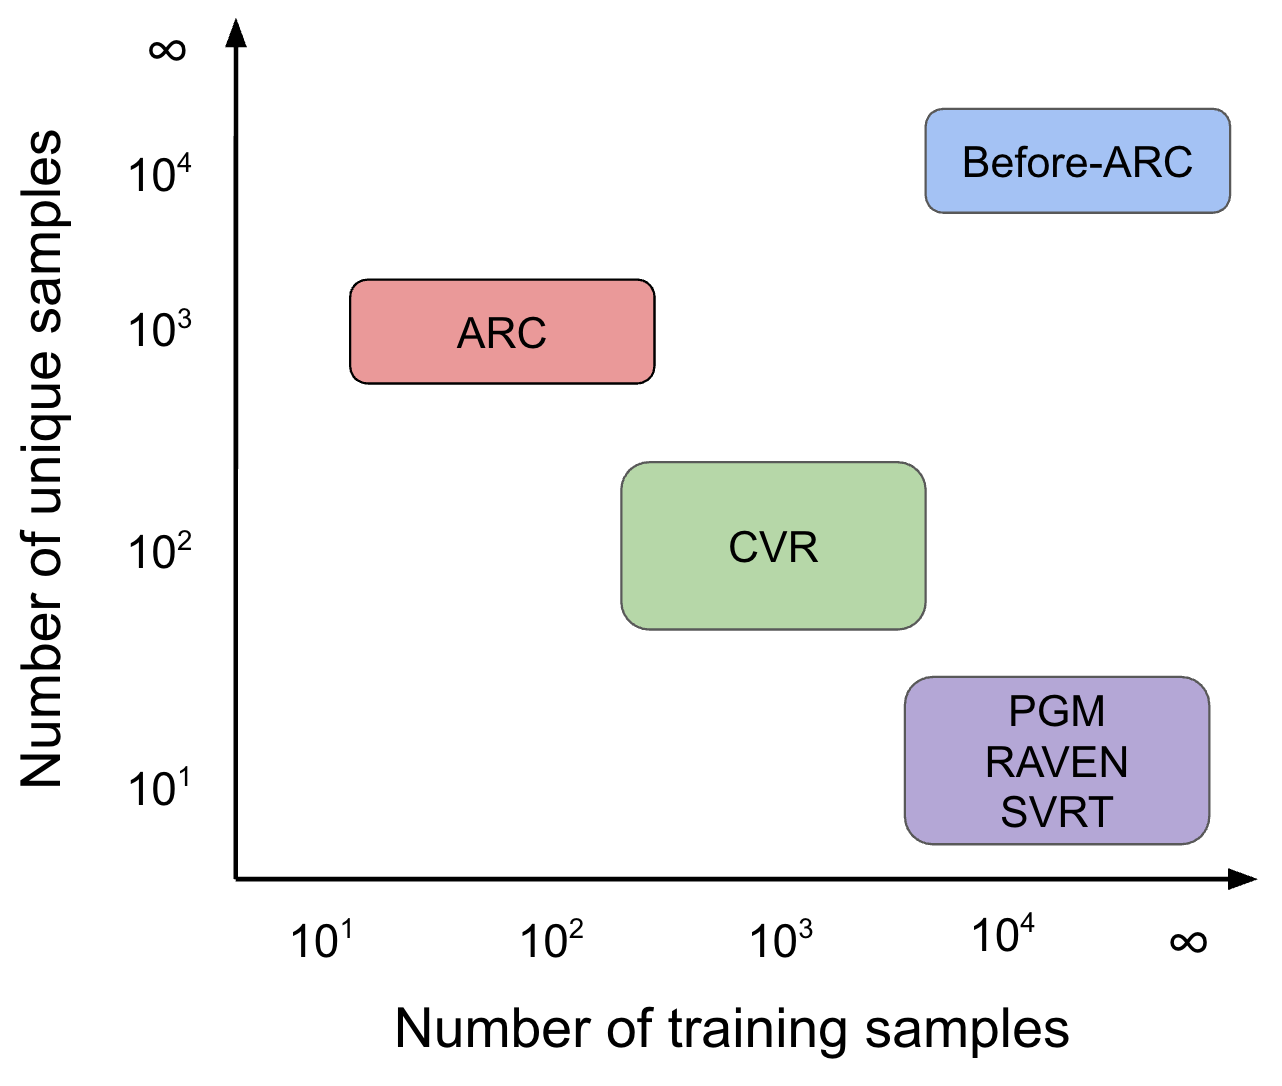
\includegraphics[width=0.6\columnwidth]{Figures/comparison.png}
%     \caption{Comparison with other SOTA datasets}
%     \label{fig:comparison}
% \end{figure}
